% ======================================================================
% main.tex -- assembled submission skeleton (IEEEtran journal class)
% Line: decoupling-marl-model-first (paper/decoupling_marl_model_first)
% Assembled mechanically from the six section drafts (2026-08-14):
%   - draft/abstract_title_candidates.md   (title + abstract)
%   - draft/introduction_sec1.md           (Section I)
%   - draft/related_work_sec2.md           (Section II)
%   - draft/methods_sec3_4.md              (Sections III-IV)
%   - draft/results_sec5_6.md              (Sections V-VI)
%   - draft/discussion_conclusion_sec7_8.md(Sections VII-VIII)
% References: working/differentiation_memo_2026-08-14.md [1]-[43]
%             (references.bib; citation-sequence by first appearance).
% No author metadata or delivery notes from the drafts are included.
% ======================================================================

\documentclass[journal]{IEEEtran}

\usepackage{amsmath}
\usepackage{amssymb}
\usepackage{graphicx}
\usepackage{booktabs}
\usepackage{cite}
\usepackage{url}

\graphicspath{{figures/}}

% Source pointers used inside captions (moving arguments): \url cannot be
% used directly in \caption, so the paths are pre-expanded with \urldef.
\urldef{\contractpath}\url{paper/decoupling_marl_model_first/working/model_contract.md}
\urldef{\pathrthreetwo}\url{results/r312_model_first_stage1/analysis.json}
\urldef{\pathrthreefour}\url{results/r344_deterministic_bridge/formal_analysis.json}
\urldef{\pathrfivezero}\url{results/r350_smooth_convex_residual/analysis.json}
\urldef{\pathrsixthree}\url{results/r363_common_channel_qp/analysis.json}

% ======================================================================
% TITLE -- PROVISIONAL, SINGLE LINE, PI-OWNED.
% PI SWAP: replace exactly the one \title line below with the final
% title wording; nothing else in the document depends on its text.
% ======================================================================
\title{An Implementation-Faithful Model-First Methodology for Storage-Coordinated Paralleled VSGs: Bounded Deterministic-Control Gain and Residual-Headroom Limits}

% ======================================================================
% AUTHOR BLOCK -- PLACEHOLDER, PENDING PI SIGN-OFF (not part of the
% section drafts; filled at submission time).
% ======================================================================
\author{\IEEEauthorblockN{Author names pending PI sign-off}%
\IEEEauthorblockA{Author affiliations pending PI sign-off}}

\markboth{Author names pending PI sign-off}%
{An Implementation-Faithful Model-First Methodology for Storage-Coordinated Paralleled VSGs}

\begin{document}

\maketitle

\begin{abstract}
Coordinating paralleled virtual synchronous generators (VSGs) with energy storage is increasingly delegated to learned controllers, but the value of a learned layer is rarely established before training compute is committed. Three obstacles block this decision: executable-plant fidelity, cross-coupled coordinates, and attribution of a negative verdict. This paper presents an implementation-faithful, gate-sequenced methodology for storage-coordinated paralleled VSGs, demonstrated end to end on a modified Kundur phasor-domain plant. A centralized deterministic controller establishes a bounded storage-power-control gain: on a sealed paired bank of sixteen scenarios it reduces the common-coordinate integral absolute error by 95.5\% and the differential-coordinate squared error by 99.3\%. The residual-headroom gate returns a bounded negative: the outcome-seeing residual upper bound reaches the registered 2\% common-endpoint floor to within $1.7\times10^{-9}$, and four causal map families under three progressively richer information configurations add no qualifying increment. An action-basis ablation completes the diagnosis: one fleet-equal common channel makes all sixteen exposed cases feasible versus ten of sixteen, identifying the zero-common residual contract, not information availability, as the structural limiter of common-coordinate headroom. The negative results are gate outcomes of the protocol, not a verdict on learning; the transferable lessons are the fidelity contract, the headroom-first decision procedure, and designing common-mode authority into the action basis.
\end{abstract}

% Keywords: provisional candidates; author must confirm before submission.
\begin{IEEEkeywords}
Virtual synchronous generator, energy storage coordination, deterministic control, residual learning, common/differential decomposition, implementation fidelity.
\end{IEEEkeywords}

\section{Introduction}
\label{sec:introduction}

Inverter-based resources are reshaping power-system dynamics, and grid interconnection standards now specify grid-forming capability and coordination behaviour for these devices \cite{ieee2800,nerc2023grid,unifi2024specifications}. Among the proposed mechanisms, paralleled virtual synchronous generators (VSGs) with co-located energy storage are a natural platform for coordinated active-power control: the storage devices provide the intervention authority, and the VSG swing dynamics provide the frequency objectives that matter for both the system-wide common mode and the relative synchronization between units. Learned control is now routinely proposed for this coordination task, from decentralized multi-agent deep reinforcement learning for multi-VSG frequency stability \cite{kang2025enhancing} and distributed multi-agent reinforcement learning for dynamic inertia-droop coordination \cite{yang2023distributed} to multi-agent learning for fast frequency response in hybrid plants \cite{ikram2026novel}, and the field has matured enough to carry dedicated surveys \cite{ding2024deep}. A study that adds another learned controller to this list would be incremental; the open question is not whether learning can be applied, but whether it should be trained at all for a given plant and baseline.

Despite this progress, three limitations persist in the way learning-based coordination evidence is produced. First, the executable plant is rarely reconciled against the intended model before results are measured: benchmarking efforts explicitly document how much fidelity work realistic grid tasks require \cite{marchesini2025rl2grid}, and the field's own surveys call for exactly the fidelity, comparator, and safety discipline that individual studies often omit \cite{yu2025safe,glover2025deep}. Second, the residual-learning premise, that a learned layer improves over a strong deterministic base, is usually assumed rather than measured: the residual family trains the correction by default \cite{liu2025residual,johannink2019residual,silver2018residual}, without first quantifying whether a residual of material size exists after the base controller. Third, when a learned layer fails to add value, the failure is rarely attributed: the evaluation literature shows how easily reported gains dissolve under seed and implementation variation \cite{henderson2018deep,agarwal2021deep}, but positive coordination studies typically do not report matched deterministic baselines or such statistical discipline. The consequence is a literature in which training-worthiness is decided by convention rather than by evidence, even though structured-learning results show that learning can beat optimized classical controllers when the conditions are right \cite{cui2023reinforcement}.

In this work we pose the training-worthiness question directly and make it the object of study. Our goal is a gate-sequenced methodology that decides, before any training, whether a bounded learned residual has physical headroom above an implementation-faithful deterministic baseline on a storage-coordinated paralleled-VSG plant, with ``do not train'' as a legitimate, pre-registered terminal decision. Two hard constraints define the problem. Every candidate arm, learned or not, must act through the same actuator map, limits, projection, and information timing as the deterministic baseline, so that a measured difference is attributable. And every verdict must be produced by a fail-closed, pre-registered gate whose thresholds cannot be relaxed after inspection.

Three challenges stand between this goal and a naive implementation. The first is fidelity: the simulator's executable device laws differ from the intended equations in ways that change measured endpoints, so the plant contract must be reconciled against source and validated by canary stages before any controller result is trusted. The second is structure: the plant is not hard-decoupled, its common and differential coordinates are measurably cross-coupled, and a distributed action basis can structurally lack authority over the very endpoint the residual is supposed to improve. The third is attribution: a negative learning verdict must separate ``there is no residual'' from ``the information path cannot see it'' from ``the action basis cannot express it'', and the information-structure literature shows these are genuinely different regimes \cite{dobbe2017fully,ho1980team}.

We address the three challenges with three methodology modules executed as one gate sequence. The implementation-faithful contract reconciles the intended equations with the executable simulator, distinguishes request, commanded, and achieved power, and terminates in nominal and signed-power canary stages (Section~\ref{sec:gate-methodology}). The coordinate contract derives an exact inertia-weighted common/differential decomposition, freezes the action basis and the deterministic baseline, and qualifies reduced models on a fresh bank (Section~\ref{sec:gate-methodology}). The diagnostic gates then answer the headroom question in three layers: an outcome-seeing offline oracle that ignores information constraints; causal map families under progressively richer neighbour information, including one-hop state and model-prediction messages; and an action-basis ablation that adds one fleet-equal common channel to the zero-common basis (Sections~\ref{sec:results} and~\ref{sec:mechanism}). Cooperative distributed model predictive control represents the alternative of extending the information path instead of gating it \cite{stewart2010cooperative,conte2016distributed,lin2024power}, and structured-learning designs represent the alternative of guaranteeing the learner rather than the baseline \cite{kwon2023risk}. Our methodology keeps both as options that the gate decides whether to open.

The methodology was executed end to end on a modified Kundur phasor-domain plant, and it returned a complete, attributable verdict. We summarise the contributions as follows. First, we present an implementation-faithful, gate-sequenced pre-training protocol for storage-coordinated paralleled VSGs, including the executable plant contract and its canary stages (Sections~\ref{sec:plant}--\ref{sec:gate-methodology}). Second, we report a bounded deterministic result and a bounded negative result from the same discipline: the deterministic baseline reduces the common-coordinate integral absolute error by 95.5\% and the differential-coordinate squared error by 99.3\% over matched zero control on a sealed paired bank, while the outcome-seeing residual upper bound stops at the registered 2\% common-endpoint floor to within $1.7\times10^{-9}$ and the tested causal families add no qualifying increment (Section~\ref{sec:results}). Third, we provide the mechanism-level diagnosis: a zero-common residual basis structurally cannot reach the common endpoint, and adding one fleet-equal common channel makes all sixteen exposed cases physically feasible versus ten of sixteen without it (Section~\ref{sec:mechanism}). Together these results demonstrate the protocol, not a learned controller: the gate established a real deterministic gain, refused training when the measured headroom could not justify it, and named the structural reason.

\section{Related Work}
\label{sec:related-work}

\subsection{Learned control of VSGs and frequency}
Deep and reinforcement learning for virtual-synchronous-generator control is an active and surveyed field \cite{ding2024deep}, driven by grid-forming specifications and interconnection standards \cite{ieee2800,nerc2023grid,unifi2024specifications}. Representative works apply decentralized multi-agent deep reinforcement learning to multi-VSG frequency stability \cite{kang2025enhancing}, distributed multi-agent deep reinforcement learning to dynamic inertia-droop coordination of paralleled VSGs \cite{yang2023distributed}, multi-agent learning to fast frequency response in inverter-based hybrid plants \cite{ikram2026novel}, reinforcement learning inside small-signal admissible ranges of VSG inertia and damping \cite{benhmidouch2024novel}, and bio-inspired multi-agent learning to islanded load-frequency control \cite{li2024bioinspired}. What this literature rarely reports is the combination this paper makes load-bearing: an implementation-faithful plant contract, a matched strong deterministic baseline under identical information, action, and limit permissions, and seed-level statistical discipline, and the two representative studies closest to this surface combination \cite{kang2025enhancing,yang2023distributed} report positive coordination claims without such a matched baseline.

\subsection{Residual and structured learning}
The residual-learning family layered a learned correction over a good-but-imperfect base controller \cite{johannink2019residual,silver2018residual}, and its power-systems instance trained deep reinforcement learning over a model-based optimization base for inverter Volt-Var control \cite{liu2025residual}. The base is named, but training is not conditional on a measured residual: the learned layer is trained by default. The structured-learning school instead engineers the learner's guarantees directly: Lyapunov-structured policies for primary frequency control \cite{cui2023reinforcement}, risk-constrained and coherency-aware learning for inverter-dominated grids \cite{kwon2023risk,kwon2024coherency}, safe reinforcement learning with stability guarantees for grid-forming frequency regulation \cite{shuai2024safe}, explicit neural networks that imitate constrained optimization inside a certified region \cite{ma2023safe}, and meta-reinforcement-learning pre-training for fast adaptation of grid-forming storage \cite{zhang2025pretraining}. These results are strong and must calibrate our claims: in particular, \cite{cui2023reinforcement} reported a structured learner that outperforms optimal linear droop, which is exactly why this paper's negative results are stated as information-path-specific rather than as a verdict on learning in general. What none of these works does is gate the training decision itself on a pre-registered, non-learning residual-headroom measurement after an implementation-faithful deterministic baseline.

\subsection{Fidelity and benchmarking}
The benchmarking stream establishes the fidelity half of this paper's contract. RL2Grid builds on the Grid2Op framework with operator collaboration, standardized tasks, operational heuristics, and safety constraints, and reports that classic reinforcement learning baselines define a reference bar that realistic tasks strain \cite{marchesini2025rl2grid}. The L2RPN challenge ran competition-grade evaluation with rule-based baselines remaining competitive and unseen-topology generalization as a first-class object \cite{marot2020learning,marot2022trust}. Adjacent comparative studies cover safe reinforcement learning against classical controllers for voltage regulation \cite{nguyen2026safe}, linear-to-learning converter control assessments \cite{wan2026comparative}, and algorithm-level deep reinforcement learning benchmarking for islanded microgrid frequency control \cite{salawuddeen2025benchmarking}. These works rank algorithms or benchmark tasks; none decides, for one plant contract, whether training should start at all.

\subsection{Evaluation discipline and information structure}
Two bodies of theory explain why a bounded negative above a strong deterministic baseline is the statistically expected outcome and how to state it honestly. The statistics-of-reinforcement-learning canon shows that reported gains shift with seeds, hyperparameters, and implementation details \cite{henderson2018deep,engstrom2020implementation}, that policy-gradient estimates can misalign with the true gradient \cite{ilyas2020closer}, that single point estimates are rarely informative \cite{agarwal2021deep}, and that simple strong baselines are systematically underestimated in multi-agent settings \cite{yu2022surprising}. The information-structure literature has shown that the amount of a centralized optimum a decentralized information structure can reconstruct is a structural property \cite{dobbe2017fully,ho1980team}, and that nonlinear policies can beat affine ones only when the information structure supplies the needed side information \cite{mehmetoglu2014deterministic,baglietto2001numerical}. Cooperative distributed model predictive control represents the ``extend the information path'' alternative: neighbour trajectory exchange approaches centralized performance under iteration \cite{stewart2010cooperative,conte2016distributed,lin2024power}. This paper sits in the cell these lines leave empty: a pre-registered, gate-sequenced training-worthiness decision after an implementation-faithful deterministic baseline, with the negative verdict attributed by design.

\section{Plant and implementation contract}
\label{sec:plant}

This section fixes the executable plant and the implementation contract that every later stage validates against; no later result is measured on a plant different from the one specified here.

\subsection{Test system}
\label{sec:test-system}

The study object is a modified Kundur two-area phasor-domain system \cite{kundur1994power} implemented in the ANDES 2.0.0 simulation framework \cite{cui2024hybrid} on a 100 MVA, 60 Hz base. It retains the four original GENROU synchronous machines with their IEEEG1 governors and EXST1 exciters, together with a low-inertia wind proxy at bus 8. Four controllable nodes are added, each composed of a network bus, a 200 MVA VSG proxy (PV + GENCLS), and a separate co-located energy storage unit (PV + ESD1). The storage units are the only actuators in this line: VSG-proxy inertia and damping are frozen plant parameters, not online actions. Table~\ref{tab:nodes} lists the four nodes; the VSG proxies have device-base $M = 200$, $D = 100$, i.e.\ system-base $M = 400$, $D = 200$ on the 100 MVA base, and the storage units are rated 36 MVA with 28 MWh energy capacity, initial state of charge (SOC) of 0.5, and SOC bounds [0.2, 0.8]. Fig.~\ref{fig:plant} shows the modified plant, the three distinct graphs, and the three power layers.

\begin{figure*}[!t]
\centering
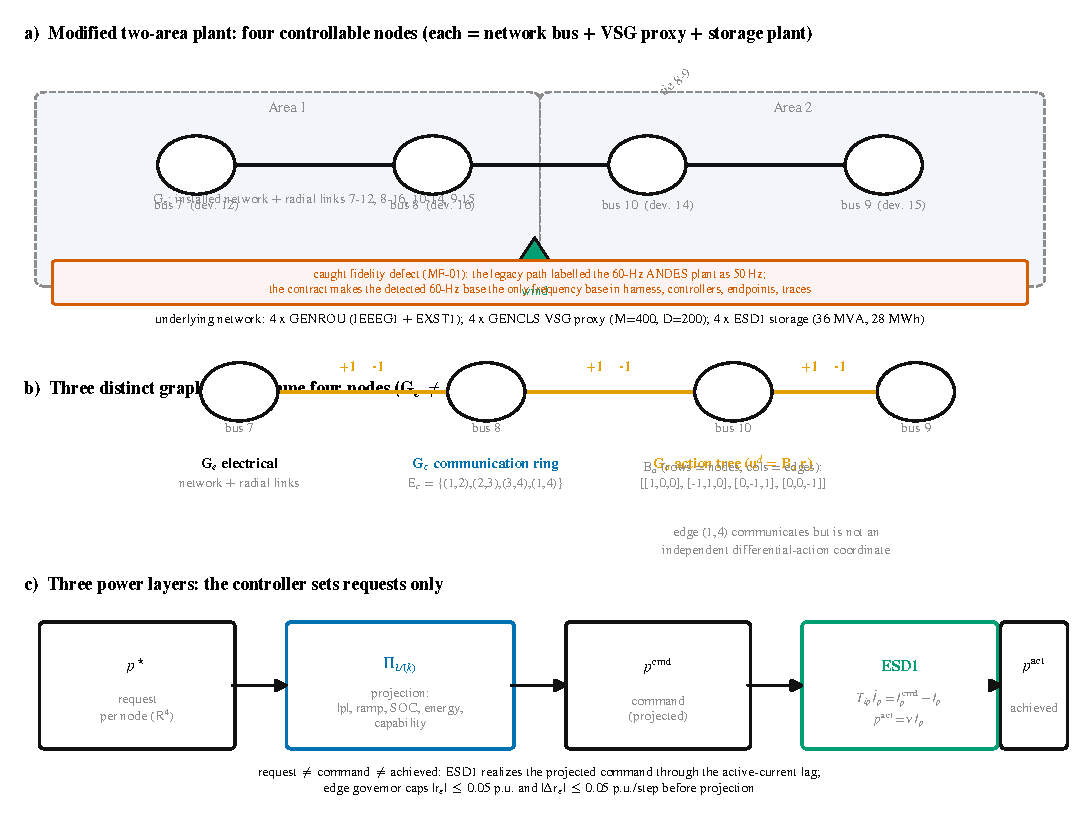
\includegraphics[width=\textwidth]{fig1_plant_contract}
\caption{The modified Kundur two-area phasor-domain plant and its implementation contract: (a) four controllable nodes, each a network bus with a GENCLS VSG proxy and a co-located ESD1 storage unit, the storage units being the only actuators; (b) the three distinct graphs kept separate in implementation and reporting --- the electrical graph, the communication ring, and the oriented active-power action tree with incidence $B_a$; (c) the three logged power layers (request, command, achieved). Source: model contract (\contractpath).}
\label{fig:plant}
\end{figure*}

\begin{table}[!t]
\centering
\caption{Four controllable storage nodes: parent network bus, device bus, and area for each VSG proxy and its co-located energy storage unit. Source: model contract (\contractpath).}
\label{tab:nodes}
\begin{tabular}{lccc}
\toprule
Node & Parent bus & Device bus & Area\\
\midrule
1 & 7 & 12 & 1\\
2 & 8 & 16 & 1\\
3 & 10 & 14 & 2\\
4 & 9 & 15 & 2\\
\bottomrule
\end{tabular}
\end{table}

\subsection{Executable device laws}
\label{sec:device-laws}

The validation truth is the sampled-data index-1 differential-algebraic equation (DAE) model (\ref{eq:dae_plant}):
\begin{equation}
E_d(\rho_k)\,\dot{x} = f(x,y;\rho_k,p^*,d_k), \qquad 0 = g(x,y;\rho_k,p^*,d_k),
\label{eq:dae_plant}
\end{equation}
where $x$ collects machine, governor, exciter, GENCLS, storage current-lag, and SOC states, $y$ the network and device algebraic variables, $\rho$ the frozen plant parameters, $p^*$ the four-dimensional storage active-power request, and $d$ the physical disturbance. Each VSG proxy follows the GENCLS swing equations (\ref{eq:gencls_swing}):
\begin{equation}
\dot{\delta}_i = 2\pi f_n(\omega_i-1), \qquad M_i\dot{\omega}_i = t_{m,i} - t_{e,i} - D_i(\omega_i-1),
\label{eq:gencls_swing}
\end{equation}
and the storage unit realizes its command through an active-current lag and achieved power (\ref{eq:esd1_lag}):
\begin{equation}
T_{ip}\,\dot{I}_{p,\mathrm{out}} = I_{p,\mathrm{cmd}} - I_{p,\mathrm{out}}, \qquad P_{\mathrm{grid}} = v\,I_{p,\mathrm{out}},
\label{eq:esd1_lag}
\end{equation}
with $T_{ip} = 0.02$ s, a voltage-dependent current path, ride-through recovery, and an SOC law with charge/discharge efficiencies 0.9848857802, all subject to the installed 60 Hz default recovery breakpoints, which are part of the validation truth rather than optional detail.

\subsection{Three power layers}
\label{sec:power-layers}

The implementation distinguishes three power layers that are all logged: the controller request $p^*$, the external command $p_{\mathrm{cmd}}$ after the repository's deterministic projection, and the achieved power read back from the plant. The projection enforces, in order, ramp (0.072 p.u./step), nameplate power (0.36 p.u.), voltage-current capability, SOC bounds, and one-step energy limits. Reporting only the request would be insufficient: the controller commands power, it does not set achieved power, and the internal storage limiters can act without appearing in the request record.

\subsection{Graphs and action basis}
\label{sec:graphs}

Four distinct graphs are kept separate in implementation and in reporting. The electrical graph is the Kundur network plus the four radial links. The communication graph is the fixed undirected ring $\{(1,2),(2,3),(3,4),(1,4)\}$. The active-power action graph is the oriented tree $((1,2),(2,3),(3,4))$ with incidence $B_a$; a tree-edge flow (\ref{eq:zero_common})
\begin{equation}
u^d = B_a r, \qquad \mathbf{1}^{\mathsf{T}} u^d = 0,
\label{eq:zero_common}
\end{equation}
satisfies $\mathbf{1}^{\mathsf{T}} u^d = 0$, so a differential-only action redistributes power among the four nodes and cannot create net fleet power. The fourth communication edge carries messages but no independent actuator coordinate. The disturbance graph records the edited PQ device or physical outage. An edge-action governor bounds each differential coordinate to $|r_e| \le 0.05$ p.u.\ with a per-step change limit of 0.05 p.u., inside the endpoint headroom and node-level projection.

\subsection{Implementation reconciliation}
\label{sec:plant-recon}

Before any result was accepted, the intended equations were reconciled against the executable simulator source, producing a repair list whose items are material to measured endpoints: the legacy observation path labelled the 60 Hz plant as 50 Hz; the GENCLS M/D write path mixed device and system bases; a default silently reduced the original G4 inertia; the storage telemetry did not expose the internal current-limiter path; and the legacy incidence sign of the inertia module is opposite to the active-power action basis. The reconciled contract, the repaired guards, and the one-sample causal timing between disturbance, command, and achieved power are frozen for all subsequent stages. These repairs are reported as part of the methodology contribution, not as peripheral software notes.

\section{Gate methodology}
\label{sec:gate-methodology}

This section defines the gate sequence as a decision procedure: every stage is pre-registered, sealed, fail-closed, and its verdict is attributable to one changed factor.

\subsection{Gate sequence and sealing discipline}
\label{sec:gate-sequence}

Every stage is a pre-registered, fail-closed gate over the unchanged plant. Each gate freezes a written contract (what changes, what is fixed, the decision tree, and the stopping outcomes) before data access; runs a rehearsal over the identical verification path; seals source and case hashes; and writes results into a create-only root that cannot be edited after inspection. A failed gate stops the route; thresholds are never relaxed after inspection, and a retry is a new prospectively registered attempt. For the physical closed-loop stage, the process budget was measured and frozen before the seal, and every worker pinned its native numerical threads to one. Fig.~\ref{fig:gate} shows the gate sequence as a decision procedure.

\begin{figure}[!t]
\centering
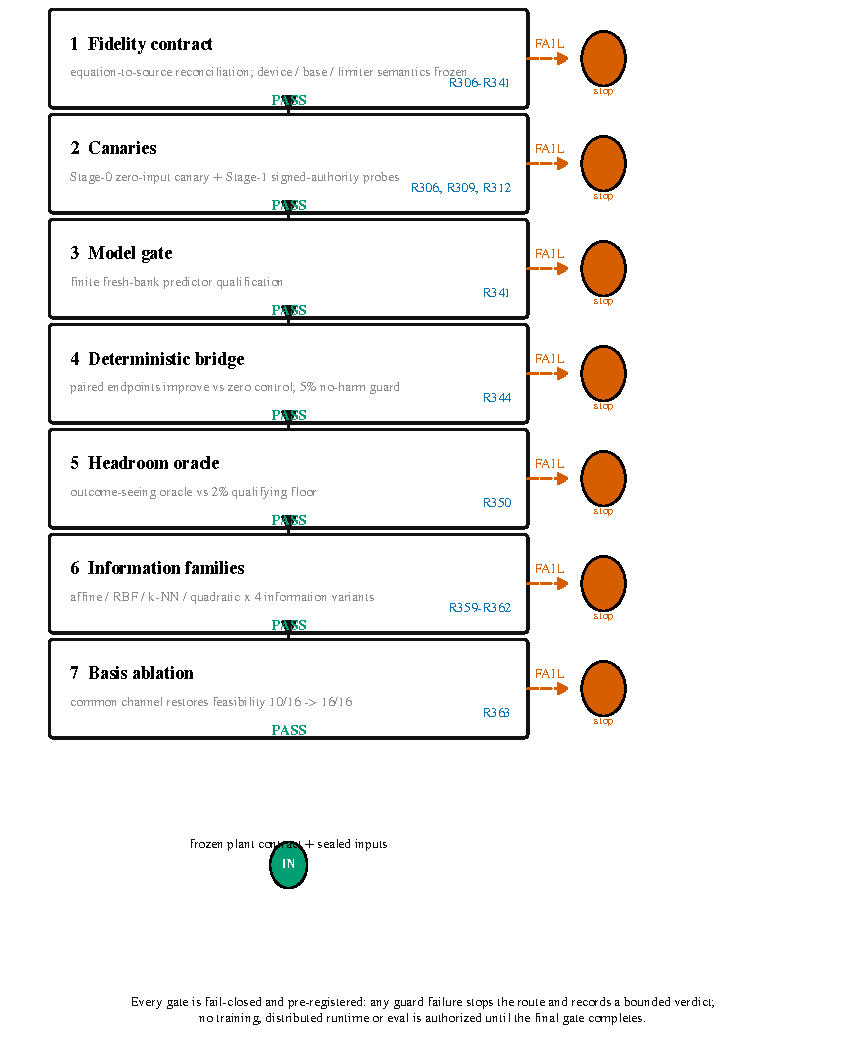
\includegraphics[width=\columnwidth]{fig2_gate_sequence}
\caption{Gate sequence of the proposed methodology: every stage is a pre-registered, sealed, fail-closed gate over the unchanged plant, and a failed gate stops the route without threshold relaxation after inspection. The terminal decision ``do not train'' is a legitimate, pre-registered outcome.}
\label{fig:gate}
\end{figure}

\subsection{Stage 0 and Stage 1 canaries}
\label{sec:canaries}

Stage 0 is a nominal readback canary: a disturbance-free five-sample trajectory with zero requests that must show power-flow and time-domain simulation (TDS) success, equilibrium DAE residual at most $10^{-8}$ (measured $2.9\times10^{-9}$), exact live system-base $M = 400$ and $D = 200$ readbacks with zero M/D write count, zero request/command/achieved power, zero SOC drift, all internal limiter variables finite, and Line\_8 in service throughout. Stage 1 applies signed active-power probes: common pulses $\pm 0.05\cdot\mathbf{1}$ and independent edge pulses $\pm 0.05\cdot b_e$ for every action-tree column, each held five samples and released for twenty. Passing requires signal-to-baseline separation of at least 20 in $L_2$, correct achieved-power sign, a final active sample within 5\% of the command, exact request-level fleet neutrality, achieved residual fleet imbalance at most 5\% of the commanded residual $L_1$ norm, monotone SOC direction, and midpoint nonlinearity ratios at most 0.25 at the OP0 point and 0.50 across all points; the measured ratios were 0.003 and 0.004. The same stage also measured the retained common/differential cross gains: across twelve coordinate/operating-point pairs, cross-to-self $L_2$ ratios ranged from 1.11\% to 3.90\%, so hard decoupling was rejected prospectively and the cross blocks were retained in every later model (Fig.~\ref{fig:probes}).

\begin{figure}[!t]
\centering
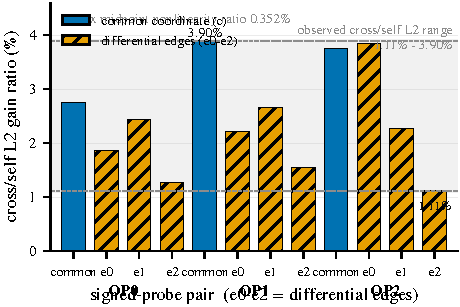
\includegraphics[width=\columnwidth]{fig3_stage1_probes}
\caption{Stage-1 signed active-power probes (R312): measured common/differential cross-to-self $L_2$ gain ratios across twelve coordinate/operating-point pairs range from 1.11\% to 3.90\%, so hard decoupling is rejected prospectively and the cross blocks are retained in every later model. Source: R312 feed (\pathrthreetwo).}
\label{fig:probes}
\end{figure}

\subsection{Coordinates and model qualification}
\label{sec:coordinates}

Control coordinates are the inertia-weighted common/differential transform (\ref{eq:coordinate_transform}):
\begin{equation}
\xi = Q^{\mathsf{T}} M_0^{1/2}\,\Delta\omega,
\label{eq:coordinate_transform}
\end{equation}
with one common coordinate and three differential coordinates; the incremental plant model is obtained by Schur complement elimination of the network algebraic variables, and control and physical-disturbance inputs are kept as separate channels
\begin{equation}
z_{k+1} = A z_k + B_u u_k + B_d d_k,
\label{eq:separate_input}
\end{equation}
rather than a shared input (\ref{eq:separate_input}). Reduced order-12 candidates were constructed at two locally defined operating points and qualified on a fresh finite bank: the registered ceilings were normalized root-mean-square error (NRMSE) at most 0.15 and peak residual at most 0.20, with worst measured order-12 NRMSE 0.130 and peak residual 0.087; the full sampled model measured worst NRMSE 0.021. This qualification is point-specific: it neither validates interpolation nor claims a general linear parameter-varying (LPV) law.

\subsection{Deterministic baseline}
\label{sec:deterministic}

The retained deterministic reference is a centralized constrained receding-horizon controller acting in the four coordinates. It uses the order-12 separate-input model, a disturbance-augmented estimator, and a direct quadratic program (QP) solve \cite{stellato2020osqp} at every 0.2 s control instant with node power (0.36 p.u.), ramp (0.072 p.u.), SOC, and energy constraints, falling back to a bounded ramp toward zero if the QP is unavailable. Its request passes through the same physical projection as every other arm. A second, endpoint-local deterministic law (linear feedback on the frequency and rate difference of each edge's two endpoints) exists and passed its own bounded holdout gate, but it is not the headline reference of this paper: the centralized controller is the upper reference, and the comparison discipline below fixes every arm's actuator map, limits, and projection.

\subsection{Residual-headroom and diagnostic gates}
\label{sec:residual-gates}

The registered endpoints are the common-coordinate integral absolute error and the summed differential-coordinate squared error over a 25-sample transient. A residual action is defined as a zero-common edge allocation $p^r = B_a r$ passed through the exact physical projection, and the residual-headroom gate asks whether any residual improves the common endpoint by at least 2\% without differential degradation and without any guard failure, i.e.\ whether the physically constrained joint-endpoint QP (\ref{eq:joint_qp})
\begin{equation}
\begin{aligned}
\min_{r}\ \bar{e}_d(r)\quad \text{s.t.}\quad & \bar{e}_c(r) \le 1 - 0.02, \quad \bar{e}_d(r) \le 1,\\
& u = B_a r, \quad (r,u,p) \in \mathcal{C}_{\mathrm{phys}},
\end{aligned}
\label{eq:joint_qp}
\end{equation}
is feasible, where $\bar{e}_c(r)$ and $\bar{e}_d(r)$ are the common-coordinate integral absolute error and the summed differential-coordinate squared error normalized to the matched zero-control baseline, $u = B_a r$ is the zero-common residual allocation through the frozen tree-edge incidence $B_a$, and $\mathcal{C}_{\mathrm{phys}}$ collects the exact physical projection limits (node power 0.36 p.u., per-step ramp 0.072 p.u., SOC bounds [0.2, 0.8], one-step energy and voltage-current limits). Three diagnostic layers make a negative answer attributable: (i) an outcome-seeing offline upper bound (smooth convex oracle) that ignores information constraints; (ii) causal per-edge map families (affine, RBF kernel ridge, 5-nearest-neighbour, and quadratic) fitted offline with leave-one-scenario-out validation over standardized 15-field endpoint-local observations, extended with one-hop state messages and with four-step model-prediction messages in two further variants; and (iii) an action-basis ablation that adds one fleet-equal common channel to the three-edge basis and re-solves the same physically constrained QP (\ref{eq:joint_qp}). These programs test whether a residual action exists; they do not define how a causal runtime controller would obtain one, and no neural network, reinforcement learning policy, or training object is involved in any of them.

\subsection{Paired evaluation discipline}
\label{sec:paired}

Every claim-bearing comparison is paired: the two arms share initialization, disturbance, timing, simulator settings, actuator path, and guards, and differ only in the registered variable (controller versus zero control; one action basis versus another; one information family versus another). The formal physical bank contains sixteen scenarios (two operating points, four active-load locations, two signs), each executed as a matched pair of 25-sample trajectories. Two zero-action and sixteen signed-authority canaries had to pass before the bank was released. A 5\% no-harm limit applies to every scenario. Holdout cases exist but remain unexamined for the headroom gates; no holdout conclusion is claimed.

\section{Deterministic baseline, residual headroom, and information families}
\label{sec:results}

This section reports the bounded deterministic gain, the residual-headroom upper bound, and the information-family gate outcomes produced by the sealed bank.

\subsection{Bounded deterministic gain}
\label{sec:deterministic-gain}

The sealed physical bank contained sixteen scenarios (two locally constructed operating points, four active-load locations, both signs), each executed as a matched pair of 25-sample trajectories (32 formal trajectories in total). Relative to the paired zero-control arms, the frozen centralized deterministic controller reduced the mean common-coordinate integral absolute error by 95.5\% and the mean summed differential-coordinate squared error by 99.3\%. Both endpoints improved directionally at both operating points, every nonzero case engaged the controller, and no scenario violated the registered 5\% no-harm limit (Fig.~\ref{fig:bridge}). As preregistered secondary diagnostics that did not enter the classifier, the scenario-mean frequency IAE fell from 0.00114 to 0.00005 Hz-s and the mean per-trajectory maximum pairwise frequency deviation fell from 0.00104 to 0.00009 Hz. These are finite-bank transient summaries over one centralized controller; they establish a bounded deterministic gain and nothing about stability, safety, distributed execution, or learning.

\begin{figure*}[!t]
\centering
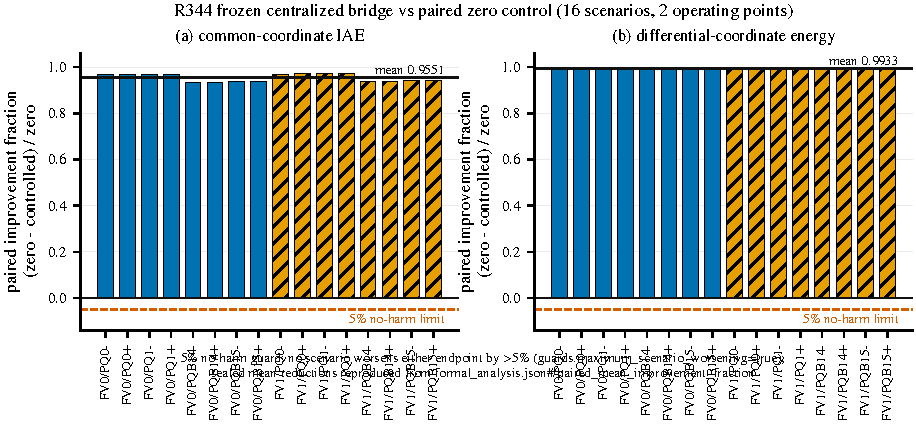
\includegraphics[width=\textwidth]{fig4_deterministic_bridge}
\caption{Frozen centralized deterministic controller versus matched zero control on the sealed paired bank of sixteen scenarios (R344; 32 formal trajectories): the controller reduces the mean common-coordinate integral absolute error by 95.5\% and the mean summed differential-coordinate squared error by 99.3\%, with every scenario within the registered 5\% no-harm limit. Source: R344 feed (\pathrthreefour).}
\label{fig:bridge}
\end{figure*}

\subsection{Residual headroom: the oracle upper bound and physical feasibility}
\label{sec:headroom}

The residual-headroom gate asks whether a zero-common three-edge residual action, passed through the exact physical projection, can improve the common endpoint by at least 2\% without differential degradation. The outcome-seeing offline oracle, which ignores every information constraint, improved the mean common-coordinate IAE by 1.9999998\%, i.e.\ $1.7\times10^{-9}$ short of the strict 2\% floor, while improving the differential endpoint by 5.1\%; the joint nominal gate therefore did not pass (Fig.~\ref{fig:oracle}). The held-out endpoint-local linear proxy, which uses only the two endpoints of each edge at the causal pre-action time, improved the common endpoint by 0.14\% and worsened the differential endpoint by 14.1\%. Both candidates also failed the mismatch-bounded endpoint gates. The frozen decision tree returned NO-TRAINING.

Two further feasibility layers bound where physical headroom does and does not exist. In the relaxed problem (the three edge actions unbounded, all physical and information restrictions removed), six of the sixteen exposed cases are certified infeasible for simultaneous 2\% improvement in both endpoints. Adding the exact physical limits to the ten relaxed-optimal cases leaves all ten accepted with zero linear, power, ramp, and SOC violations and a minimum SOC margin of 0.235, i.e.\ per-case physical action-space headroom exists in ten of the sixteen exposed cases, while six remain infeasible even in the relaxation.

\begin{figure}[!t]
\centering
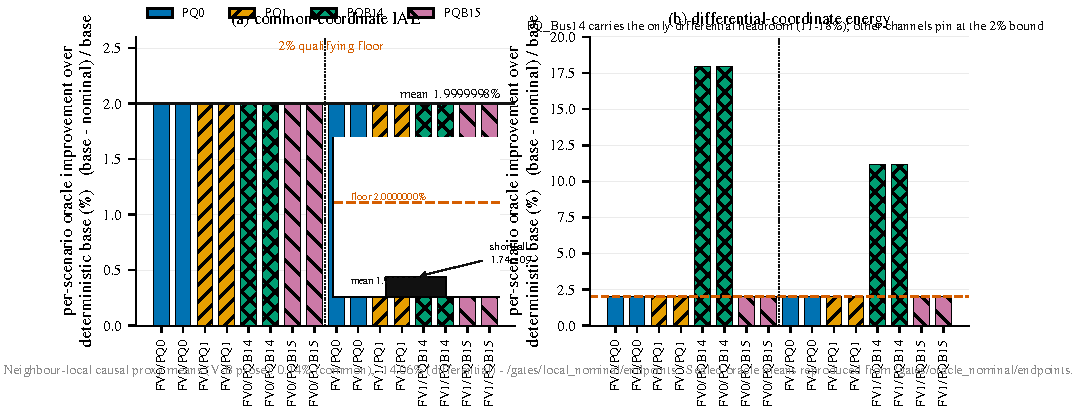
\includegraphics[width=\columnwidth]{fig5_oracle_headroom}
\caption{Outcome-seeing residual-headroom oracle (R350): the offline oracle improves the mean common-coordinate integral absolute error by 1.9999998\% ($1.7\times10^{-9}$ short of the strict 2\% floor) while improving the differential endpoint by 5.1\%; the endpoint-local linear proxy improves the common endpoint by only 0.14\% and worsens the differential endpoint by 14.1\%. The joint nominal gate does not pass. Source: R350 feed (\pathrfivezero).}
\label{fig:oracle}
\end{figure}

\subsection{Information families}
\label{sec:families}

Four pre-registered, tuning-free causal map families (fixed affine, RBF kernel ridge, 5-nearest-neighbour, and quadratic polynomial) were fitted per edge with leave-one-scenario-out validation and passed through the exact physical projection. The gate was run over three progressively richer information configurations: 15-field endpoint-local observations (snapshot), tested with the affine family and with the three nonlinear families; the same 15 fields plus one-hop neighbour state messages (23 fields); and four-step model-prediction messages from the two ring neighbours replacing the snapshot messages. No family cleared either endpoint group in any configuration. Table~\ref{tab:family} reports mean nominal common-coordinate improvement (2\% paired gate) and the differential mean signed relative change, where values above 1 denote worsening.

The mismatch-bounded endpoint groups failed for every family in every variant as well. Every integrity check passed in all four gates, so these failures are gate outcomes of the frozen contracts, not data defects. The results reject only the tested families under the frozen contracts; they establish no claim about neural policies, which were never trained or evaluated anywhere in this line.

\begin{table*}[!t]
\centering
\caption{Information-family gate outcomes: mean nominal common-coordinate improvement (percent; the 2\% paired gate) and differential mean signed relative change (multiplicative; values above 1 denote worsening) for each tested family under the three registered information configurations. No family cleared either endpoint group. Source: R359--R362 feeds.}
\label{tab:family}
\begin{tabular}{lccccc}
\toprule
Variant & Affine & RBF & 5-NN & Quadratic\\
\midrule
Snapshot, common & 0.50\% & 0.92\% & 0.89\% & 1.11\%\\
Snapshot, differential & 6.12$\times$ & 14.56$\times$ & 5.80$\times$ & 36.93$\times$\\
One-hop messages, common & 1.06\% & 1.01\% & 0.79\% & $-0.95\%$\\
One-hop messages, differential & 0.94$\times$ & 19.81$\times$ & 5.05$\times$ & 142.74$\times$\\
Prediction messages, common & 0.68\% & 1.15\% & 1.29\% & $-0.06\%$\\
Prediction messages, differential & 3.78$\times$ & 32.68$\times$ & 4.85$\times$ & 672.93$\times$\\
\bottomrule
\end{tabular}
\end{table*}

\section{Mechanism diagnosis: the zero-common action basis as structural limiter}
\label{sec:mechanism}

This section reports the action-basis ablation that attributes the negative headroom verdict of Section~\ref{sec:results}.

The information-family negatives leave open whether the residual premise fails because of information or because of the action basis itself. A zero-common edge residual satisfies $\mathbf{1}^{\mathsf{T}} p^r = 0$: it redistributes power among the four nodes and carries no fleet net power, so the common endpoint can only be improved indirectly through cross-coupling. The mechanism gate extended the frozen three-edge basis with one fleet-equal common residual-power channel, the four-channel node-action basis $[\mathbf{1}, B_a]$, and re-solved the identical physically constrained joint-endpoint QP (\ref{eq:joint_qp}) on the same sixteen exposed development cases. All sixteen cases became physically feasible, versus the ten-of-sixteen three-edge baseline, and every one of the six previously infeasible scenarios was unlocked (Fig.~\ref{fig:common}). In every feasible case the common-coordinate ratio reached 0.0000--0.0002 (the registered 2\% improvement achieved with essentially the entire common endpoint removed) with zero differential degradation and zero physical-limit violations.

This is an information-unconstrained physical feasibility statement: it shows that the zero-common residual contract itself, not information availability, is the binding structural constraint on common-coordinate headroom. The common endpoint cannot be reached through zero-sum edge channels alone, while a fleet-equal channel removes it directly. It does not establish that any information path or learning method can select the common channel, it does not overturn the information-family negatives, and it authorizes no controller or learning conclusion. The result also breaks the fleet-neutrality assumption of the earlier residual contract: any successor formulation must re-derive the power/energy contract before execution claims are possible.

\begin{figure*}[!t]
\centering
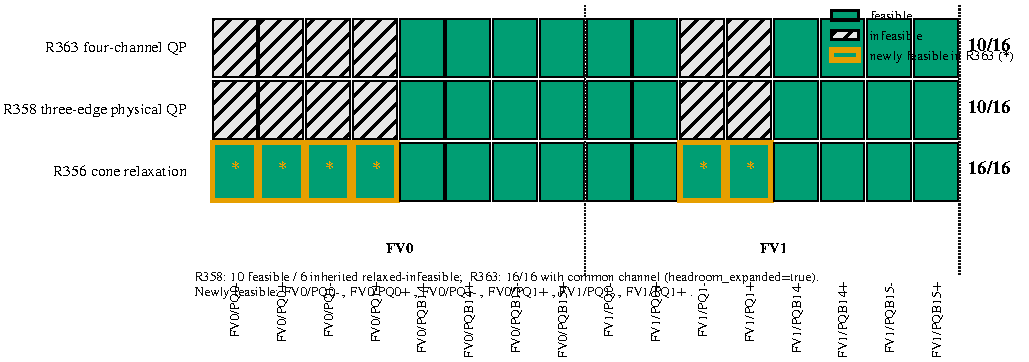
\includegraphics[width=\textwidth]{fig7_common_channel}
\caption{Action-basis ablation (R363): extending the zero-common three-edge residual basis with one fleet-equal common channel makes all sixteen exposed cases physically feasible versus ten of sixteen without it, unlocking every previously infeasible scenario. The zero-common residual contract, not information availability, is the structural limiter of common-coordinate headroom. Source: R363 feed (\pathrsixthree).}
\label{fig:common}
\end{figure*}

\section{Discussion and limits}
\label{sec:discussion}

This section states what the diagnostic chain licenses and what it refuses, and enumerates the exact scope of every reported number.

\subsection{What the diagnostic chain says, and what it does not}
\label{sec:what-it-says}

The three diagnostic layers make the negative verdict attributable rather than anecdotal. The outcome-seeing oracle shows that almost no nominal residual value remains after the deterministic controller: the outcome-seeing offline upper bound reaches the 2\% common-endpoint floor to within $1.7\times10^{-9}$ and no further. The information-family gates then show that the tested causal maps, with progressively richer neighbour information, cannot even approach that bound without degrading the differential endpoint. The action-basis ablation finally shows where the headroom went: a zero-common basis structurally cannot touch the common endpoint, and one fleet-equal channel removes it almost entirely. The bottleneck is therefore the residual contract's action basis, not the information path. This is the mechanism-level lesson of the paper: before training a distributed learned residual, verify that the reserved action basis still carries authority over the endpoint the residual is supposed to improve.

Two disciplined readings are rejected. The negative family results do not establish that residual learning is impossible or useless in general: they reject only the four tested tuning-free families under the frozen contracts on one plant, and no neural policy was ever trained or evaluated. Nor does the common-channel result establish that a learning method can select the common channel under causal information; it is an information-unconstrained feasibility statement. The common channel also breaks the fleet-neutrality assumption that the deterministic contract reserved for itself, so any successor formulation must first re-derive the power and energy contract.

\subsection{Scope of every reported number}
\label{sec:scope}

Every quantitative statement in this paper is a finite-bank transient summary: one modified Kundur phasor-domain topology, two locally constructed operating points, four active-load locations with both signs, 25-sample transients, offline linear-response maps for the headroom gates, and a centralized deterministic controller. The headroom results read no holdout cases. The result archive is local and not publicly pushed. The paper therefore claims no stability certificate, no safety argument, no robustness outside the registered bank, no topology generalization, no EMT, HIL, or deployment evidence, and no conclusion about any simulator other than ANDES 2.0.0. These are not rhetorical hedges; they are the exact boundaries the sealed gates enforced.

\subsection{What transfers conceptually}
\label{sec:transfers}

Three design lessons transfer independently of the specific plant. First, an implementation-faithful contract with canary stages converts simulator defects into caught failures instead of silent evidence: the repairs listed in Section~\ref{sec:plant-recon} changed measured endpoints and would have invalidated any unchecked study. Second, the headroom-first sequence (deterministic baseline, outcome-seeing upper bound, causal map families, action-basis ablation) is a reusable decision procedure that returns an attributable answer before training compute is committed. Third, zero-sum distributed action bases cannot reach fleet-common endpoints; common-mode authority must be designed in or consciously excluded from the start. What does not transfer is every measured number and every controller: they are evidence for this plant and this frozen contract only.

\section{Conclusion}
\label{sec:conclusion}

This paper presented an implementation-faithful, gate-sequenced methodology for storage-coordinated paralleled VSGs and demonstrated it end to end on a modified Kundur phasor-domain plant. The implementation contract reconciled the intended equations with the executable simulator and its canary stages validated the actuator path before any controller result was accepted. Under this discipline, the sealed paired bank produced a bounded deterministic gain and a bounded negative: the controller reduced the two registered endpoints by 95.5\% and 99.3\% over matched zero control, the outcome-seeing residual upper bound stopped at the 2\% common-endpoint floor to within $1.7\times10^{-9}$, and the tested causal map families added no qualifying increment under any of the three registered information configurations. The action-basis ablation completes the diagnosis: extending the zero-common three-edge basis with one fleet-equal common channel makes all sixteen exposed cases physically feasible versus ten of sixteen without it, identifying the zero-common residual contract, not information availability, as the structural limiter of common-coordinate headroom.

The negative results in this paper are gate outcomes of the proposed protocol, not a verdict on learning in general. The positive contribution is the protocol itself: it established a real deterministic gain, caught its own fidelity defects, refused training when the measured headroom could not justify it, and named the mechanism. For the next study, the operational lesson is direct: design common-mode authority into the action basis, and re-derive the power and energy contract before any residual layer is trained.

\section*{Acknowledgment}
Generative AI tools were used to assist drafting, copy-editing, and review of this manuscript; every scientific statement and numerical result was produced from and verified against the authors' experimental records, and the authors take full responsibility for the content. % AI-tool disclosure: author must confirm wording, name the tools used, and state the sections and level of assistance before submission.
% Funding statement: author to complete.
% Conflicts of interest: author to complete.

\bibliographystyle{IEEEtran}
\bibliography{references}

\end{document}
